\documentclass[a4paper]{article}

%% Language and font encodings
\usepackage[english]{babel}
\usepackage[utf8x]{inputenc}
\usepackage[T1]{fontenc}
\usepackage{CJKutf8}

%% Sets page size and margins
\usepackage[a4paper,top=3cm,bottom=2cm,left=3cm,right=3cm,marginparwidth=1.75cm]{geometry}

%% Useful packages
\usepackage{color}
\usepackage{amsmath}
\usepackage{graphicx}
\usepackage[colorinlistoftodos]{todonotes}
\usepackage[colorlinks=true, allcolors=blue]{hyperref}
\usepackage{amsfonts}
\usepackage{amssymb}
\pagenumbering{gobble}
\usepackage{verbatim}
\usepackage{setspace}
\usepackage{mathtools}

% Keywords command
\providecommand{\keywords}[1]
{
  \small	
  \textbf{\textit{Keywords---}} #1
}


\title{Retirement expectations under pension reforms: How do old Europeans respond to increases in legislated retirement ages?}
\author{Jiadi Cong}

\begin{document}
  \maketitle

\begin{abstract}
This paper investigates how old individuals’ retirement expectations response to the increases in either normal retirement ages (NRAs) or early retirement ages (ERAs) issued between 2011 and 2013. Using repeated data from two waves of the Survey of Health, Ageing and Retirement (SHARE), we find that the effect of increases in ERAs are substantial, amounting to 5.98 percentage point increase in the subjective probability of continuing working after age 63. Increases in NRAs do not seem to have such average effect. However, results suggest that workers have increased their entitlement of alternative pension plans to counteract the changes in NRAs. 
\end{abstract}

\keywords{Pension reforms, early retirement, retirement expectations.}

\doublespacing

%remember to reset to 1.0

\section{Introduction}

Increasing longevity and trend of early retirement are undermining the sustainability of the social welfare state in many of the European countries (Siegrist et al. 2007). In combination with the decreasing fertility, the public pension systems based on a pay-as-you-go (PAYG) scheme will hardly maintain retirement income adequacy. Since the last decades, governments across Europe have reduced the generosity of early retirement benefits or raised the legislated retirement age to increase public awareness of individual responsibility (OECD 2013). Yet, in most European countries the effective retirement age is still below the legislated age of normal retirement. To determine whether these pension reforms are effective in altering actual retirement patterns, it is important to investigate their impact on individuals’ retirement expectations, which reflect not only the future retirement inclinations but also people’s current financial preferences (Coppola and Wilke 2014). 

The present paper refers to the increases in normal retirement ages (NRAs) and early retirement ages (ERAs) in Europe issued during 2011 to 2013. The new pension policies have required individuals, for instance, to contribute additional years to obtain retirement eligibility, or to retire at a higher statutory retirement age. Regardless of the detailed institutional settings, each of the reforms have strived to reduce the rate of early retirement in certain age cohorts, that is, individuals of other age cohorts are unaffected. These reforms therefore provide a quasi-experimental framework. Because individuals cannot choose their birth date, we are able to exploit the causal effect of the pension reforms. 

We first employ a non-stochastic lifecycle budget constraint framework to model behaviors under changes of legislated retirement ages. As NRA increases, the model predicts that a new bunching of retirement will be observed at the post-reform pension age, while the share of the new bunching is decreased. Furthermore, an aggressive increase in NRA can possible trigger escapes from normal retirement plan to an earlier retirement scheme, especially for individual who values leisure more relative to consumption. In the case of ERA increase we show that the share of the new bunching depends on the relative change between NRA and ERA. 

Using data from the Survey of Health Ageing and Retirement in Europe (SHARE) collected in 2011 and 2013, we measure the effect of increase in the legislated retirement ages on two aspects of individuals’ retirement expectation: subjective probability of working after 63, which reflect the expectation of job exit; and expected pension age, which reflect the expectation of pension benefit collecting. We first address the general trend of individuals’ retirement expectation by plotting the survival curve of workers’ expected pension age both before and after the reforms. The followed quantitate analyses suggest that the reforms in ERAs significantly raise individuals’ working intention. In particular, the subjective chance of working after 63 is on average 5.98 percent higher for those with increased eligible ERA. Changes in NRAs do not have such average effect, but it raises the subjective likelihood of working beyond age 63 for the high-educated cohorts by 6.59 percent. The findings are consistent with the predictions of our lifecycle labour supply model, which reminds the policy makers that strong reforms in NRA may push workers into alternative benefit plans. This statement is also supported by examining the changes in entitlement of plans other than public normal pension plan. We furthermore exploit the quantile effects to interpret whether individuals with different retirement preference at baseline respond differently to the reforms. Results indicate that individuals who are not certain about their retirement plan at baseline have stronger responds to shifts in ERAs.

The contribution of this paper is two-folded. First, we providing quantitative evidence on the effects of reforms on elder’s (aged over 50) retirement expectation across 10 European countries. Using an international microdata set is preferred as it provides variation in pension systems and individual level conditions (Fischer and Sousa-Poza 2006). Moreover, within-country studies are usually facing restriction in number of observations, which may lead to potentially biased estimation (e.g., Coppola and Wilke 2014). Second, while past studies only analysis sole change in pension system, we reveal individuals’ responds to simultaneous increases in both NRA and ERA. To our knowledge, this paper is the first to theoretically and empirically examine assorted changes in pension age across Europe using individual level data.

The remainder of this paper begins with a brief review of the changes in NRAs and ERAs in Europe during 2010 to 2013. Later sections present a lifecycle labour supply model, survey data, empirical strategy and the treatment analyses, followed by heterogeneity check. This paper concludes with policy recommendations. 
\section{Pension reforms}

Public pension reforms during 2011 to 2013 in Europe are signals on how governments plan to extend people’s working lives. As pension systems differ by country, the reforms may also vary, but overall have taken on three forms, namely: 1) raising the legislated NRA; 2) tightening the early retirement pathways; and 3) increasing financial incentives to retire late (OECD, 2015). Through the last strategy increases the opportunity cost of early exit, the actual change in benefit is difficult to measure as benefit schedules are highly diverse by country. This following part thus set out the most salient changes through the first two forms.

  \subsection{Raising the NRAs} 
  
  In Denmark and Estonia, new reforms are phased based on previous pension reform issued in the period of early 21th century. Specifically, in Denmark the increase in NRA was brought forward, starting from 2013 and have reached to 67 years in 2017. The NRA will increase to 65 by 2026 for both gender in Estonia. Before 2011 in many Western European countries, the full pension age has reached to a stable state, generally at 65 years for both genders (in Italy at 60 for women).  During 2011 to 2013 new pension legislation in France, Netherland and Spain were announced to increase the full pension age to 67 years, at different speeds. In Italy, the NRA has increased for women from 60 to 66 years, to match that of men by 2018 (OECD 2013). Before 2011, retirement age in the Czech Republic is correlated with the number of children. Announced in 2011, a progressive increase of two months (four months for women) each year of the NRA would start from 2013. Since the magnitude of increase will accelerate to six months from 2019, the exact pension age for women will become less depended on the number of children they have had and will uniformly reach to 66 years and eight months, unified with men’s pension age. In another Eastern European country, Slovenia, the NRA will increase to 65 for men and 63 for women in a four-year interval, from 2021 to 2024. To sum up, these reforms in general include a two or more years’ increase in NRA and are comparatively more aggressive with women. The trend is clear that most of the European countries have converged normal pension age of both sexes to a same level. Only Slovenia, in our study, still have different ages for the two genders by 2028.  

  \subsection{Tightening the early retirement schemes} 
  
  Early retirement was initially introduced to be use mainly by heavy physical or high dangerous labour, and as means of creating new jobs (Velladics et al. 2006). In recent decades, however, the scheme has created overwhelming financial burden for European public security systems. During 2011 to 2013, strict reforms have been adopted to reduce early-withdraws from the labour market. In the Western European countries, Belgium, Denmark, France and Spain, the eligible age for early entitlement to retirement benefit has increased, up to 65 years. In Italy the 2011 reform abolished the former system under which individuals can retire at 61 if satisfied 35 years of contribution. Workers who enrolled in the scheme before the reform are still possible to retire from age 62, with at least 42 contributed years (41 years for women).  In the Czech Republic and Estonia, age for early pension has increased at a same speed as of the NRA. In addition, in Austria, Belgium, France, Italy and Spain, eligibility for early retirement has become more dependent on a worker’s employment history. Stricter requirement has been applied on the number of years that individuals has paid social security contribution, known as the “contribution years”. Comparatively, expect a half-year increase in France, contribution years for full normal pension was unchanged in the studied countries during 2011 to 2013. As a summary, for those who have entitled to a public retirement plan, the state retirement age reforms during 2011 to 2013 are universal across most age cohorts and occupations. One salient pattern is that simultaneous changes in NRA and ERA are prevailing. This trend of reform is further interpreted by a static labour supply model, as discussed in the following.  

\section{A life-cycle labour supply model of retirement decision}

In this section we introduce a non-stochastic life-cycle budget constraint model referring to the one presented by Burbidge and Robb (1980), to capture the effects of retirement age changes and to generate predictions for the retirement behavior. The model provides a framework to interpret individual’s trade-off between retirement leisure and consumption in the presence of both legislated NRA and ERA and gives a visual estimation of the retirement planning with policy intervention, therefore motivate the further empirical analysis.

Individual concerned in this model is able to choose her retirement age freely, meaning that she cannot be forced to leave the labour force by illness, layoff or other reasons. Assume that the individual makes her retirement decision in period “0” with a wealth of $W_0$ and will live for $T$ more periods with certainty. She will spend R years working full-time with a fixed income of Y and then spends the rest of her life $(T-R)$ periods in retirement. To simplify, we assume no payroll tax and the interest and discount rates are equaled to zero. Individual’s preferences are defined over consumption and retirement leisure, therefore the utility function has the form $U(C(t),v_t L(t))$. The term $L(t)$ in the model, which stands for the retirement leisure, is only available in her retirement periods as 1, and takes the value as 0 when she is still in working periods. The term $v_t$, which is the coefficient before the leisure term, measures the relative value of leisure compared to consumption and is associated with individual characteristics including age, health status and gender (Gustman and Steinmeier 2005).

The individual can choose from two social benefit plans: normal and early retirement schemes. Both of the plans provide pension benefits, $P^n$ and $P^e$ respectively, starting from the period of retirement and smoothly cover the rest periods of her life. In reality, the eligibility of retiring through normal or early retirement pathways can be obtained by satisfying a required year of contribution to the plan as well as reaching the legislated age of retirement. As most of the pension benefits are closely related to the accrual rate generated by each year of contribution, the normal retirement plan would therefore provide better benefits than early retirement plan, as $P^n>P^e$. We assume that individual can no longer opt into normal retirement plan after retired through early retirement plan. If the utility function is concave to the original point, the individual concerned will maximize her overall utility subject to her lifetime budget constraint as represented following:

\begin{equation}
\operatorname{Max}_{C(t), R} \int_{0}^{R} U(C(t), 0) d t+\int_{R}^{T} U\left(C(t), v_{t}\right) d t
\end{equation}

subject to

\begin{equation}
\int_{0}^{T} C(t) d t=W_{0}+\int_{0}^{R} Y d t+\int_{R}^{T}\left[P^{e} \cdot \mathbf{1}\left(R^{e} \leq t<R^{n}\right)+P^{n} \cdot \mathbf{1}\left(t \geq R^{n}\right)\right] d t
\end{equation}

where $R^e$ stands for legislated ERA while $R^n$ stands for legislated NRA. $1(.)$ is an index function and takes value of $1$ if $t$ locates inside specific time intervals. For any given value of $R$, one can solve the optimal control problem with respect to $C$, which gives the result $U_c (C(t),0)=U_c (C(t),v_t )$. This implies that the marginal gain of utility in working period by one unit increase in consumption equals the marginal utility gain in retirement period by one unit increase in consumption, thus individual will perfectly smooth her consumption over the life-cycle to maximize overall utility.  Let $U^w≡U(C(t),0)$ and $U^r\equiv U(C(t),v_t )$, therefore we have ${U_C}^w={U_C}^r≡U_C$. Under the smooth consumption assumption, the individual will behave to maximize her utility as to maximize the Lagrange function with respect to $C$ and $R$: 

\begin{equation}
\begin{aligned} \operatorname{Max}_{C, R}(L)=& \int_{0}^{R} U(C(t), 0) d t+\int_{R}^{T} U\left(C(t), v_{t}\right) d t \\ &-\lambda\left\{\int_{0}^{T} C d t-W_{0}-\int_{0}^{R} Y d t\right.-\int_{R}^{T}\left[P^{e} \cdot \mathbf{1}\left(R^{e} \leq t<R^{n}\right)+P^{n} \cdot \mathbf{1}\left(t \geq R^{n}\right)\right] d t \} \end{aligned}
\end{equation}

By solving the first order conditions we have:

\begin{equation}
U_{C}^{w}=U_{C}^{r} \equiv U_{C}=\lambda
\end{equation}

\begin{equation}
\frac{U^{r}-U^{w}}{U_{C}}=\left\{\begin{array}{ll}{Y} & {\text { if } t<R^{e}} \\ {Y-P^{e}} & {\text { if } R^{e} \leq t<R^{n}} \\ {Y-P^{n}} & {\text { if } t \geq R^{n}}\end{array}\right.
\end{equation}

The left-hand side of equation (4) presents the marginal utility of one more period in retirement over the marginal utility gain of another consumption, or put it another way, the marginal rate of substitution between retirement leisure and consumption. On the right-hand side of equation (4) we have three different slops of the budget constraint based on age (or $\frac{dC}{dR}$). Before $R^e$ (or ERA), individual faces a slope of budget constraint equals to $Y$ as she will not get any pension benefit if retire before the ERA. If she continues to work after reaching the ERA, the slope will reduce to $Y-P^e$ as she forgoes the pension benefits of the additional periods of working. If the individual chooses to work beyond the NRA, $Y-P^n$ will be the new slope of her budget constraint. Note that since $P^n>P^e$, the budget constraint curve will have a concave shape towards the original point, with kinks at the two legislated retirement ages. In equilibrium, the marginal rate of substitution must equal to the slope of the budget constraint. 

Following Burbidge and Robb’s graphical analysis, we build our framework inside $C$, $T-R$ space. As illustrated in Figure 1 panel A, the slope of budget constraint in this case changes as mirror symmetry since $\frac{dC}{(d(T-R))}=-\frac{dC}{dR}$. We should assume, generally, that very few individuals would exit the labour force earlier than the ERA. This is based on the setting that there exist no pension plans other than the mentioned two in this model. With this setup, the model predicts bunching of retirements at the two legislated retirement ages as the reduction in slope after the kink points in the budget constraint. Individuals who would retire latter than the legislated retirement age in absence of social benefit, find it optimal to switch to retire at the legislated retirement age. Nonetheless, individuals with smaller  $v_t$ – preference of leisure over consumption – would still work beyond the legislated retirement age.

\begin{figure}[h] 
    \centering
    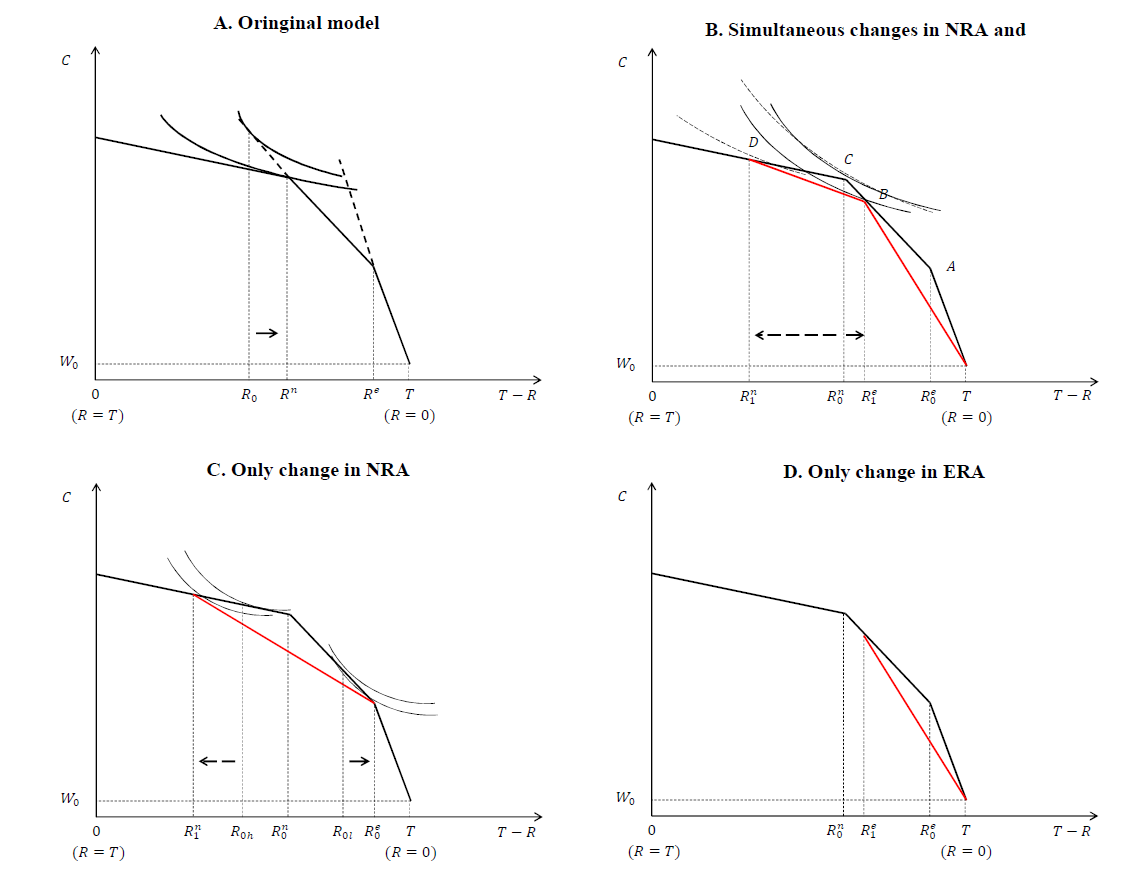
\includegraphics[width=1\linewidth]{Figure1.png}
    \caption{A non-stochastic labour supply model}
    \label{1}
\end{figure}

\subsection{Simultaneous increase in NRA and ERA}

Here we consider increases in both ERA (from $R_0^e$ to $R_1^e$) and NRA (from $R_0^n$ to $R_1^n$). The increases in legislated retirement ages lower the overall working income, as individuals have to prolong their working years to achieve the statue of retirement. However, income effect is not the same for each period. Suppose an individual retires at the decision period “0” before the pension reform, none of the increases in legislated retirement ages will decrease her lifetime income as she has zero period of working since period “0”. Likewise, for individuals who planned to retire at age equal or higher than the post-reform NRA (or $R_1^n$), the budget constrains remain unchanged as the increase in legislated retirement ages does not propose any change to her planned retirement age. Along the x-axis from $T$ to $R_1^e$ (or from $R_1^e$ to $R_1^n$), the income effect first accelerates, reaching maximum at the pre-reform retirement age, and then decelerates to zero when reaches the post-reform retirement age (measured by the vertical distance between the black curve and red curve in Figure 1 panel B). 

In Figure 1, panel B presents the geometric results as both legislated retirement ages increased. Firstly, for the increase in NRA, the model predicts that bunching shifts from the pre-reform NRA, $R_0^n$, to the post-reform NRA, $R_1^n$. For individuals who planned to retirement after the pre-reform NRA, their retirement age will prolong to the new NRA. However, the new kink at  $R_1^n$ is flatter as the slope of the budget constraint decreases for the interval between $R_1^e$ and the $R_1^n$, therefore the cluster is less concentrated compared to pre-reform era. The reason behind is that for the individuals whose indifference curves are comparatively more convex, one-unit loss in retirement leisure would take many more units of consumption to compensate for maintaining a same level of utility. This implies that if governments want to make the new NRA as attractive as the original one, subsidies must be applied, for instance, by raising the accrual rate to pension benefit.  

Second, for the increase in ERA the model also predicts a shift of bunching of retirement from $R_0^e$ to $R_1^e$. In this case, however, the share of the new bunching is uncertain as the income declined in both periods before and after the post-reform ERA. Given any new ERA say $R_1^e$, sharper increase in NRA will result in a higher level of cluster at $R_1^e$ as the greater decline in income afterward it generated, and vice versa. To be more specific, assume we have a given pension system ($R_0^e$,$R_0^n$,$P^e$,$P^n$) and individual income is known to be $Y$. From Figure 1, we derive the conditional relation of $R_1^e$ and $R_1^n$ as following:

\begin{equation}
    \frac{P^{n \prime}-P^{e \prime}}{P^{e}}=\left(\frac{P^{n}}{P^{e}}-1\right)\left(\frac{R_{1}^{n}-R_{0}^{n}}{R_{1}^{n}-R_{1}^{e}}\right)+\frac{R_{0}^{e}}{R_{1}^{e}},
\end{equation}
where $P^e$ and $P^n'-P^e'$ are given by:

$P^e$: Pre-reform cost of working beyond $R_0^e$;

$P^n'-P^e$': Post-reform cost of working beyond $R_1^e$. 

The left-hand side ratio of equation (6) is the relative cost of the working beyond the post-reform ERA. Given $R_1^e$, an increase in $R_1^n$ will raise the relative cost of working beyond new ERA. The model therefore predicts that raising NRA may trigger individual opt out from normal retirement pathway they may find the new ERA a more appropriate retiring timing.  

\subsection{Solely increase in NRA or ERA}

We investigate the effect of solely change in legislated retirement age as illustrated in Figure 1 panel C and D.  Similar to the previous analysis, the model predicts that the bunching shifts from the original retirement age to the new retirement age, but with a lower share in both cases. Notably, we expect individuals who plan to retirement at higher ages to have better chance to respond to the NRA/ERA changes, while individuals who planned lower retirement age may even be pulled from early retirement because of the forthcoming drop of yearly income. 

\subsection{Hypotheses}
Based on the presented models, we make the following hypotheses, and each of those will be tested by the followed empirical study:

$H_1$: Individuals with small $v_t$ will choose to work longer as respond to increase in ERA;

$H_2$: Individuals with large $v_t$ may have less significant or even negative respond (choose to retire earlier) to increase in NRA/ERA;

Note that past studies have assumed that merely few individuals exit the labour force before reaching ERA, which is however, not applicable in this paper. In fact, in many European countries, individuals can exit the labour market even before reaching ERA with the help of the unemployment insurance to bridge the gap years. Also, opposites to other existing studies, our model predicts that if increase in NRA is too aggressive, a group of workers may opt into an alternative benefit plan (e.g., unemployment or sick leave benefits) to bridge the years between job exit and legislated pension age, as we shall test in the empirical analysis. 

\section{Empirical data}

Our empirical analysis is based on data from the fourth (2010-2011) and fifth (2013) waves of Survey of Health Ageing and Retirement in Europe (SHARE). This is an annual panel household survey across 27 European countries and Israel that collects information on the social and financial situation, health and employment status of individuals aged above 50 years (Komp 2017). Importantly, it includes the monthly birth date of all individuals, leading us able to calculate their exact legislated retirement age. In this paper, we select the sample in three steps. First, we select those countries that had at least one reform in pension ages during 2010-2013. This allows us to include ten countries in the analysis: Austria, Belgium, the Czech Republic, Denmark, Estonia, France, Italy, the Netherland, Slovenia and Spain. Secondly, we select individual with at least one public pension account, who participated in both 2010-2011 and 2013 waves of survey. For pragmatic convenience, individuals that were self-employed at the baseline are excluded as self-employment is likely to be embedded in different institutional backgrounds, which would increase the complexity of analysis (Preter et al. 2012).  Finally, we pool 4320 repeated respondents from both waves, which give us a final sample of 8640 observations.

In this paper we use individual’s subjective probability of working full-time beyond age 63 as our main dependent variable to measure the changes in retirement preference. A question was asked to all employed individuals below or at the age of 61 at the time of interview: “Thinking about your work generally and not just your present job, what are the changes that you will be working full-time after you reach age 63?” Responses are scaled from 0 to 100 where 0 means “absolutely no chance” and 100 means “absolutely certain” that they will be working full-time after reaching age 63.  Earlier studies based on HRS (Health and Retirement Study) have suggested that the subjective probability of retirement is informative when studying the effect of policy changes. The subjective probability varies not only over employed individuals but also across waves within respondent, whereas a binary indicator of retirement does not (McGarry, 2004).  Furthermore, by observing the continuous outcomes we can study the distributional variation based on the quantiles they belong to. 

We also introduce the “expected pensionable age” as an indicator of expectation in pension benefit collection. In SHARE, individual’s expected pensionable age was collected from the following question asked of all individuals who were not yet retired: “At what age do you yourself expect to start collecting this pension (the pension you will be entitled to) payment for the first time?” In our case, the distribution of expected pensionable ages at baseline year is dominated by “spikes” at 60 and 65, usually the ages at which women or men first become eligible to collect public pension benefit. After the reforms we find a significant drop in age 65, whereas the pensionable age of beyond 65 increased moderately.

\subsection{Choice of control group}

Under individual perspective, retirement expectation is based on the current legislation of the future retirement conditions. Assuming perfect information, any departure from one’s originally expected future retirement conditions, say, an increase in pension age or serve year requirement, would evoke adjustment of her current retirement preference. Following this strategy, we first identify the impact of increases in legislated retirement ages, by calculating the legislation differences of the earliest NRAs/ERAs between 2013 and 2011 at individual level. Afterward, we identify the impact of increases in contribution year requirement, by calculating the ‘feasible’ retirement ages of those who have to work full-time beyond the legislated pension age in order to retrieve retirement eligibility. In SHARE, individuals were asked about their contributed years to public pension. Usually for the 50+ individuals, the reported years of contribution would include the periods of caring for children, as a majority of European countries give credits to this form of labour-market absences. However, it may or may not contain the periods of severe disability or unemployment, which would be used as a technique for the elders to bridge the gap between job exit and pension age. In this way, the feasible retirement age actually measures individual’s expected pension age. We should remind that the increase in contribution year requirement for early retirement in a group of countries is sharp and substantial. Consequently, individuals’ actual feasible ERAs might go far beyond the post-reform ERA as the increase in required contribution year dominants. 

Figure 2 displays the distribution of the changes in the feasible earliest NRA/ERA. From the left panel one can see that more than half of our sample is unaffected by NRA reforms, while for the affected individuals the increased expectation is clustered between “0.5” and “2”. On the other side, the increase in the feasible ERA are more separately distributed across point “0.5” to “5”, with a spike in “2”. Despite of the difference, in both cases the dominance of zero is prevailing. Therefore, it is reasonable for us to refer individuals with zero increase in the feasible NRA as the “control group in normal retirement reform” and similarly refer individuals with zero change in the feasible ERA as the “control group in early retirement reform”, while the rest serves as two separated treatment groups respectively. Note that as reforms in NRAs and ERAs are simultaneous, overlaps between different treatment or control groups may exist.

\begin{figure}[h] 
    \centering
    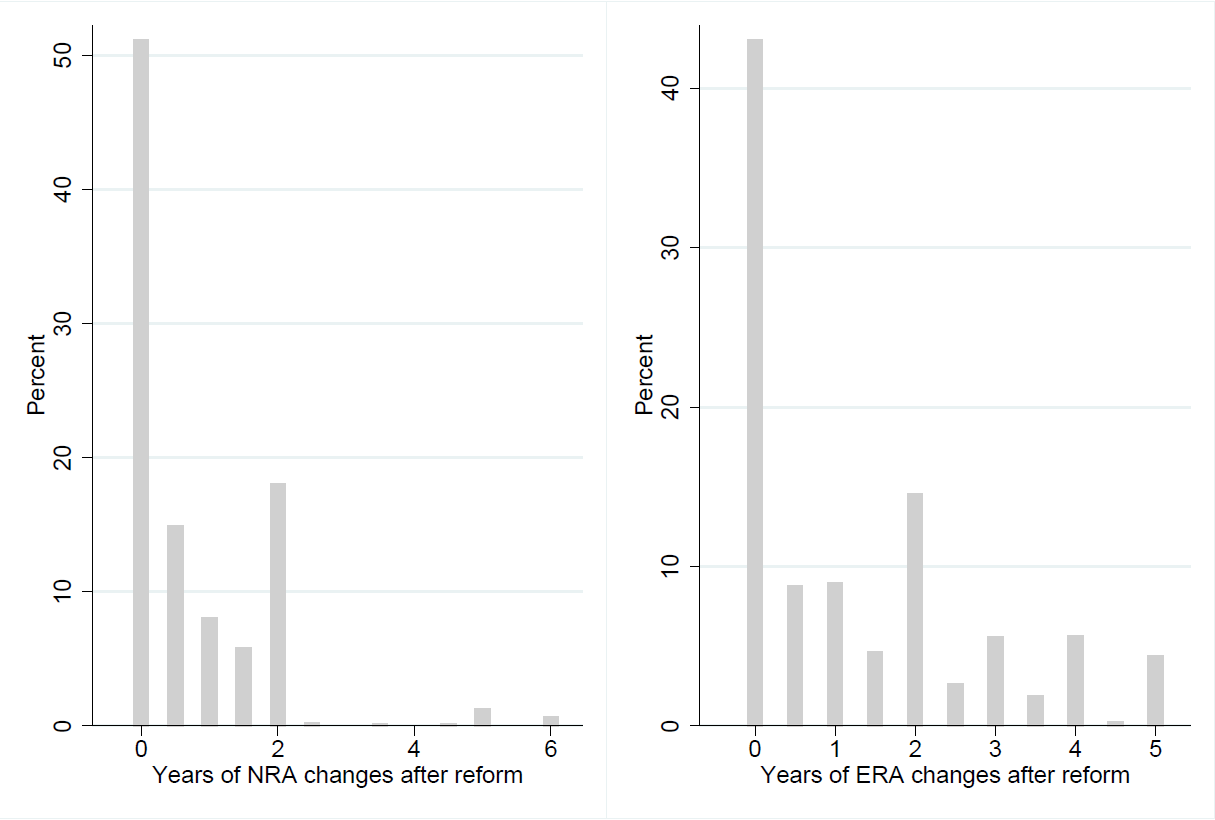
\includegraphics[width=1\linewidth]{figure2.png}
    \caption{Distribution of year of changes in NRA/ERA }
    \label{2}
\end{figure}

Many of the past studies have used self-employed individuals, who are by definition not affected by the reform as their control groups (Bottazi et al. 2006; Grip et al. 2013; Coppola and Wilke 2014). However, the unaffected assumption of self-employment is not likely to hold in this paper because of the universal coverage of public (or semi-public) pension scheme in countries such as Belgium, Denmark and the Netherlands. Some other papers studied reforms of a once-for-all increase in retirement age in European countries such as Germany and Italy. They recommended of using the older age cohorts as control group, which is yet not appropriate in our analysis. Based on our sample, 21 percent of the individuals aged above 59 have at least one-year increase in legislated NRA. In addition, countries such as Belgium have adopted immediate jumps in ERA or years of contribution required for workers of all ages. Elders would therefore very likely to experience an increasing ERA. 

Our identification strategy has the following advantages: First, we can identify individuals affected by a step-wise increase in retirement ages. Most of the past papers in effect of pension reforms only studied the effect of a once-for-all increase in retirement age, whereas most of the recent increases in legislated retirement age are step-wise. Second, we can separately examine the policy influence of normal or early retirement reforms since we introduce two separate treatments. This is crucial as the recent pension reform in one specific European country usually includes increases in both NRA and ERA. Only controlling one aspect of the reforms would create bias in estimation. Third, we calculate the feasible earliest NRA/ERA to contain the effect of changes in contribution year requirement. Since to increase the required years of contribution for early retirement is one major technique to restrict early retirement, it is rational to assume that individuals will take consideration of the change in their early retirement eligibility. 

\subsection{Treatment group vs. control groups}

Table 1 describes the distributions of individual’s subjective probability to work full-time beyond 63 at 2011 and 2013. Overall, the reported probabilities are clustered into “0s”, “0.5s” and “1s”. At baseline (year 2011), the average probability for NRA control group is equal to 0.423, greater than 0.406, the mean of the treated individuals. The same pattern follows in ERA changes, with a similar magnitude of difference (0.429 vs. 0.403). However, we find a significant deviance in the moving pattern of individuals’ subjection retirement expectation between the two treatments in 2013. Specifically, the treated and controlled groups under NRA changes both show a greater desire of working after 63 in the post-reform era (year 2013). On the other hand, the average subjective probability of treated individuals under ERA changes increases from 0.403 to 0.443, whereas that of the controlled group drops from 0.429 to 0.399. If look closely at the distribution of the ERA control group, one can see substantial increase in “absolute no chance” as well as decline in “50-50 chance” in the post-reform era. This result indicates that in absence of policy shifts, as individuals become older, they are more certain about their retirement expectation. Notably, only 31 percent of workers give identical probabilities between waves.

\begin{table}[h] 
    \centering
    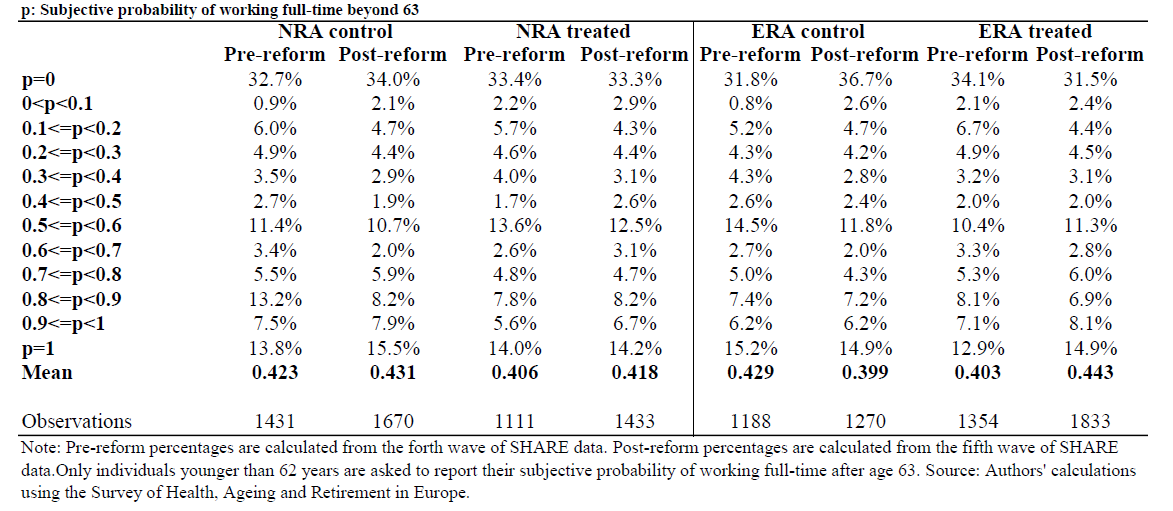
\includegraphics[width=1\linewidth]{table1.png}
    \caption{Distribution of subjective probability to work full-time beyond 63}
    \label{1}
\end{table}

\subsection{Empirical Strategy}

To reveal the effects of the pension reforms, we estimate a difference-in-differences (DiD) model of each individual’s subjective retirement probability with treatments of normal and early retirement reform. As for the concern of possible endogeneity of the reforms, we confirm that, except the gender and age differences, almost all changes in retirement age from 2011 to 2013 in Europe were implemented equally through different cohorts. An exception is the reform in Italy issued in 2011, which solely increased the NRA of women who works in public sectors. However, it is harmless to ignore the bias since the affected population only takes up 1.0 percent of the total respondents. For the age cohort and gender differences, we further examine the heterogeneity by adding the interaction dummies into the regression model.  

In order to identify the estimator in DiD model, ‘common trend’ assumption, that is, assumption of constant time effect across groups must be satisfied. Though unable to prove the assumption, Table 2 gives some useful insights by presenting the descriptive statistics for control groups and treatment groups. Despite the substantial variation in gender, there are only small differences of other characteristics between the different groups for either reform. The similarity of composition between group supports for the assumption that the treatment and control group are likely coming from a same distribution. Further, we run a placebo regression between 2006 and 2011 when there were no reforms in legislated retirement ages. After controlling the individual social-economic factors, the coefficient of policy-time interaction term is insignificant for both placebo normal and early retirement reforms (see Table A1). This result therefore stands for the assumption that without the pension reforms the subjective retirement probability of individuals in treatment and control group shares a similar trend. Then we are safe to use a linear model to implement the DiD estimators, states as follows:
\begin{equation}
\begin{aligned}p_{it}&=\alpha+\beta_1 postreform_{it}+\beta_2 NRAchange_{it}+\beta_3 ERAchange_{it} \\ &+\beta_4 NRAchange_{it}\times ypolicy_{it}+\beta_5 ERAchange_{it}\times postreform_{it}+\eta X_{it}+\epsilon _{it},
\end{aligned}
\end{equation}
where $p_{it}$ is the subjective probability of working full-time beyond 63 for individual i at time t, $postreform_{it}$ is a dummy identifying year 2013, the period after the reforms, $NRAchange_{it}$ is a dummy equal to one if the individual is identified to be affected by reform in NRA, $ERAchange_{it}$ is a dummy equal to one if individual is identified to be affected by reform in ERA and $X_{it}$ is a set of control variables. The coefficients of the two product terms $\beta_4$ and $\beta_5$ are our main interest of analysis. 

For the continuous outcomes we estimate equation (6) using ordinary least squares, with clustered standard errors at individual level. Notably, estimation bias may occur when  $ε_{it}$ contains important variables that change over time and in that way alter individuals’ retirement preference. In order to investigate, assume that rational individual adjusts his/her retirement expectation based on the arrival of new information; therefore, we check individual level shocks that are unrelated to the pension policies. Among the full sample, 1.3 percent reported change in marital status, of which 24.4 percent is due to the mortality of spouse; 8.9 percent reported a substantial change in self-rated health condition and 7 percent individuals reported mortality of natural parents in 2013 survey. We conduct t-tests on the difference of subjective retirement probabilities between individual with and without the policy-unrelated shocks, finding none of the null hypothesizes of “no difference” can be rejected. In other words, the retirement preference of individuals with policy-unrelated shock does not show significant difference to that of individuals without the shock. 

\begin{table}[h] 
    \centering
    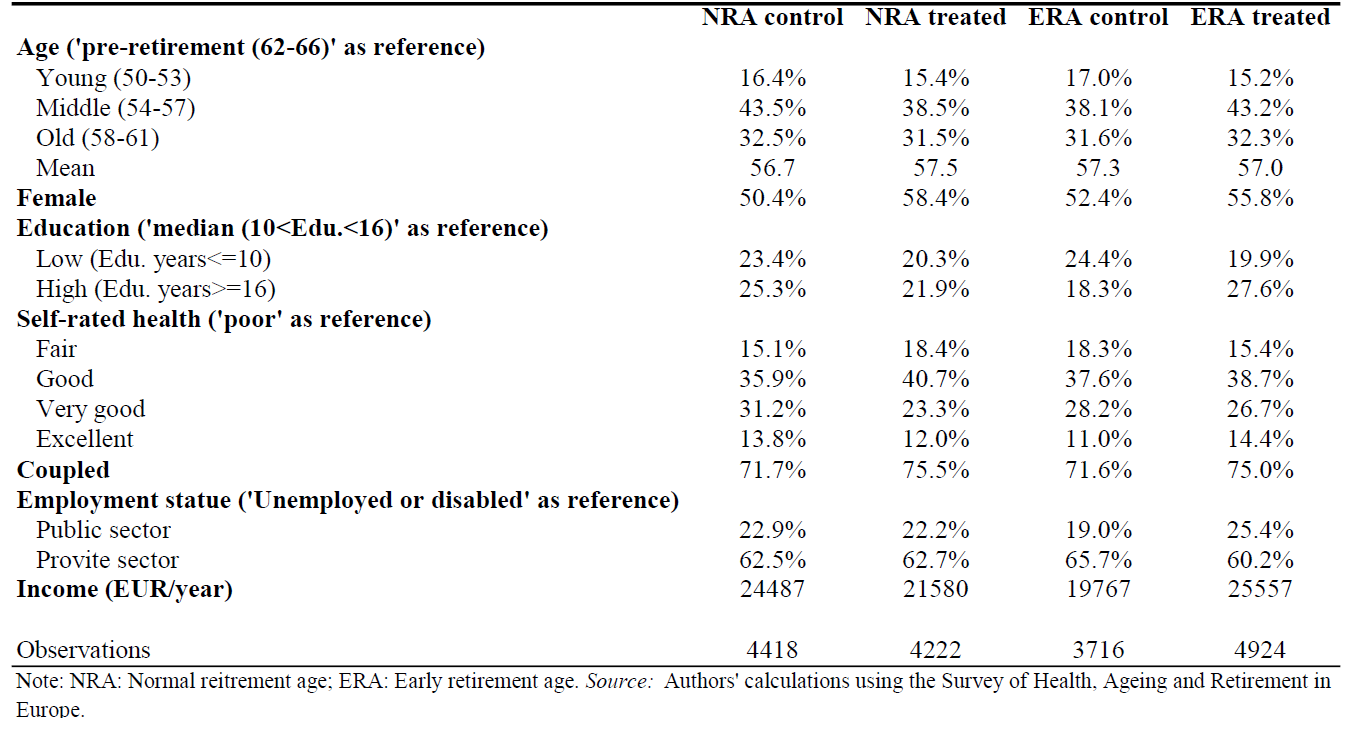
\includegraphics[width=1\linewidth]{table2.png}
    \caption{Descriptive statistics of the full sample}
    \label{2}
\end{table}
 
The covariate variables $X_it$ in the DiD model should control for the differences between groups that are not affected by the pension reforms, therefore we include variable related to individual’s sociodemographic status, employment status and health conditions. Specifically, we include country dummies (use “Austria” as reference), gender dummy, age, self-rated health condition (five levels from “poor” to “excellent”), partnership status dummy at time of interview (use “never married/divorced/widowed” as reference), education level dummies, employment status dummies at time of interview (works for private sector or public sector) and annually income. Notably for measure of education level, individuals who reported less than 11 years of education are grouped as of “low education level” while individuals with more than 15 years of education is labeled with “high education level” and the remains contribute to the “medium education level” group as reference. Table 3 provides social-eco statistics separately for the four groups at baseline (year 2011). 48.9 percent of our sample faces NRA changes, while 57.0 percent of the observations faces ERA changes. There are, unsurprisingly, a greater proportion of female workers experiencing changes in both NRA and ERA. Additionally, individuals of lower education or serving at a public sector are more likely to have an increased ERA. With respect to other individual characteristics, the distribution indicates consistent structures across four subgroups. 

In this paper, we also argue that the size of the policy effect is likely to be unequal over the scale of the subjective retirement probability. It is reasonable to assume that individuals that have low probability or “absolute zero chance” of full-time work beyond age 63 would have less respond to policy shifts since leisure would be a necessary good for them. Although studying distributional treatment effect is becoming common in recent empirical papers, as far as we know, none of the research have done it in the context of retirement reform. In this paper, we support our argument by estimating several quantiles in the distribution of the subjective probability of work full-time beyond 63 using full-set of covariates. Following Callaway and Li’s identifying assumption of treatment (2015), we estimate the quantile regression estimator which $\hat{\beta_q}$ minimizes the following objective function:
 
\begin{equation}
Q\left(\beta_{q}\right)=\sum_{i : p_{i t} \geq \boldsymbol{x}^{'}_{i} \beta}^{N} q\left|p_{i t}-\boldsymbol{x}^{'}_{i} \beta_{q}\right|+\sum_{i : p_{i t}<\boldsymbol{x}^{'}_{i} \beta}^{N}(1-q)\left|p_{i t}-\boldsymbol{x}^{'}_{i} \beta_{q}\right|,
\end{equation}
where $ \beta_q$ is the coefficient of the qth quantile.

\section{Results and discussions}
\subsection{Main estimation results}

We now examine the quantitative effects of the changes in state pension ages on workers’ subjective retirement expectations. The estimated impact on the expectation of work beyond age 63 are all estimated using DiD models, with a summary of key parameters reported in Table 3. All standard errors reported are clustered at individual level in order to account for the within personal variation. The main variable of interest here is the interaction terms between the period dummy and the NRA/ERA treatment dummy. We find the results are consistent in different models. Focusing on the results for the full covariates, the effect of increases in ERAs are substantial, amounting to 5.98 percent increases in the average subjective probability of working after age 63. However, the increases in NRAs do not seem to have such average effect. These results speak in favor of the effectiveness of ERA reforms in increasing old worker’s short-term desire to prolong their working life, while at the same time indicate the reforms in NRA on average have less effect in altering individual’s retirement expectation in short term. The different result between treatments is likely due to the stricter reforms in early retirement policies. During 2011 to 2013, many European countries have adopted sharp increase in early retirement requirement. These reforms, moreover, often come together with abolishing of some early retirement pathways, therefore may largely alter individuals’ retirement preference in short term. Consequently, on average individuals may incorporate the reforms in ERA in their retirement expectation faster compared to increase in NRA.

\begin{table}[h] 
    \centering
    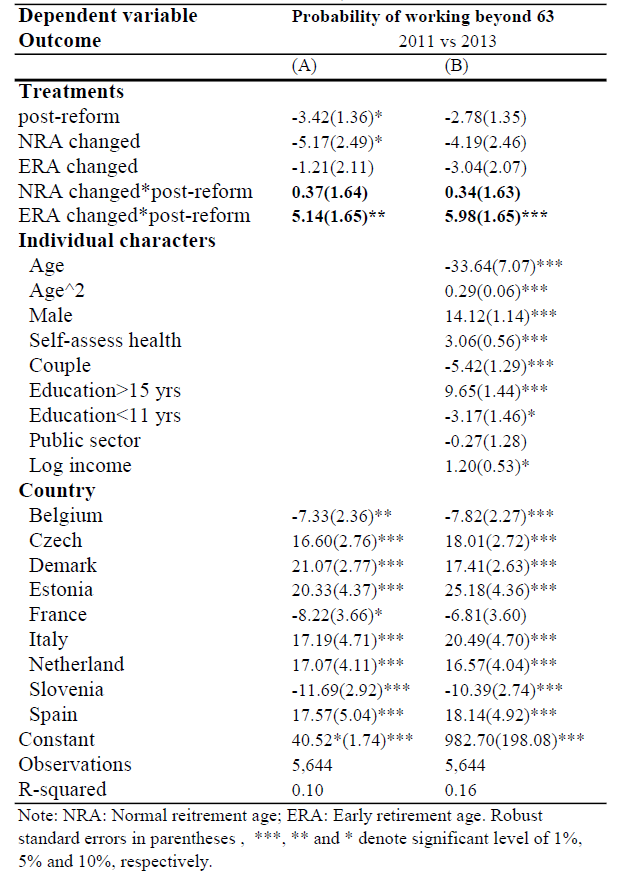
\includegraphics[width=0.7\linewidth]{table3.png}
    \caption{Difference-in-differences estimates, main results}
    \label{3}
\end{table}

\subsection{Socio-economic factors}

We find most of coefficients of the individual covariates have consistent signs with the results of related studies on the determinants of subjective retirement expectations. First, as increasing of age level, the subjective probability of working beyond 63 initially decreases, but begin to rise after reaching age 58. Male workers have on average 14.12 percent higher chance of working after age 63 than female workers do. Further, individuals with better health condition or higher education level have greater willing to work longer, while partnership decreases the work chance by 5.42 percent. Occupation in public sectors however, has no significant effect on individual’s desire to work after 63. Annually income as a presenter of individual’s financial condition has positive impact on individual’s retirement expectation. The coefficient indicates that each percent increase in income will cause 1.2 percent increase in subjective probability to continuing work beyond age 62. 



\subsection{Education, gender and age}

\begin{table}[h] 
    \centering
    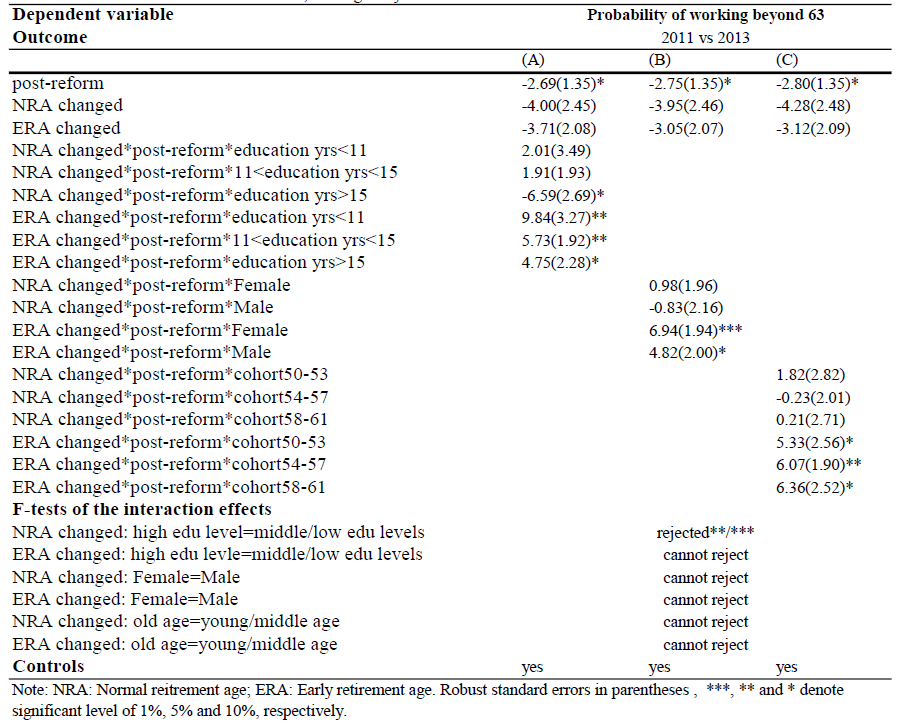
\includegraphics[width=1\linewidth]{table4.png}
    \caption{Difference-in-differences estimates, individual level heterogeneity effects}
    \label{4}
\end{table}

The analyses above show a significant effect of reforms in ERAs on individuals’ retirement expectation. In this section, we reveal some heterogeneity in the way retirement preferences respond across education level, gender and age cohorts, with results shown in Table 4. Focusing on the education aspect first (Column A in Table 4), we find that individuals of all education level have significantly response to changes in ERA, where the individuals of lower education are of greater respond. The difference in magnitude however, after conducted to an F-test, is found to be not significantly away from zero. On the other hand, the subjective probability of high-educated treatment group declined as response to the increase in NRA. A followed F-test additionally confirms the coefficient is significantly different from that of the lower education level groups. This could because individuals of better educated are usually those who have the knowledge and access of information to make strategic changes (Grip et al. 2013). In reality, as the eligible retirement age for each year is ever increasing, choosing to retire after age 63 can result in a much later NRA. For those who want and able to stick at their original planned retirement age (usually those who are also entitled in other pension plans), a tightening of normal retirement may result them in switching to an alternative scheme of lower retirement age. The results so far have supported the first three hypotheses in the labour supply model section.

Gender heterogeneity is another frequent studied factor in terms of pension reforms. Consist to a list of past studies (Staubli and Zweimu:ller 2011 ; Grip et al. 2013), we find the early retirement reforms have a more significant impact on women’s retirement expectation than man’s (Column B in Table 4). However, the followed f-tests reveals that the gender heterogeneity is not significant. On the other side, after the NRAs increased, male workers’ subjection probability of working beyond age 63 declined by 0.83 percent, while for the female the probability increased by 0.98 percent. These responds, however, are small and insignificant, indicating that both genders are insensitive to increase in NRAs in short term. Nonetheless, the opposite signs of the gender cross-term coefficients reveal a widely recognized phenomenon that female workers have a lower probability of early retirement (Dorn and Sousa-Poza 2005b; Fischer and Sousa-Poza 2006), even facing stricter retirement requirements (Grip et al. 2013). 

Turning to the age aspect, we estimate the interaction effects across three age groups, presented in Column C of Table 4. The results show that the all cohorts respond to the ERA changes by a 5.33-6.36 percent increase in the subjective working probability. Statistically no difference among the responds of the three age cohorts is detected. On the other hand, increases in NRAs has little effect on altering the retirement expectation of all three cohorts in short term. While these results give us the impression that workers of different age cohorts respond symmetrically to increases in the state retirement ages, we further conduct a heterogeneity check of the reform effects on the ‘even-older’ cohorts, namely workers aged from 62 to 66, which is defined as the ‘pre-retirement’ cohort in our analysis. Recall that in SHARE, only workers aged from 50 to 61 are asked about their subjective probability of working beyond age 63, therefore we use the ‘expected pension age’ to measure individuals’ retirement expectation in this case. The results show that the increase in NRAs reduces the expected pension age for the ‘pre-retirement’ cohort significantly (by 11 months). This is likely driven by the inability to claim normal retirement pension. For ‘pre-retirement’ cohort, a 6.7 percent of additional entitlement in social benefits other than the public normal pension is found in year 2013. On the other hand, being affected by the ERA reform is found to have increased the ‘pre-retirement’ cohort’s expected pension age by approximately 9 months on average. In both cases, the hypothesis of no difference between respond of the ‘pre-retirement’ cohort and other age cohorts are rejected at 1 percent level of significance. To deepen our understanding, we further conduct a linear treatment analysis on how individuals’ entitlement of non-public pension responds to changes in NRAs and ERAs, with the results presented in Table 7 in the latter section. Unsurprisingly, raising in NRAs have increased the likelihood of entitlement to other pension by 19 percent, suggesting a tendency of covering the loss by alternative benefits. The result explains the potential adjustment mechanism of how individuals respond to NRA increases, that is, by exiting the job market before the post-reform NRA and bridge the gap years with other security benefit. We find no significant evidence that increases in ERAs have such effect. 


\subsection{Physically demanding jobs and job satisfaction}

\begin{table}[h] 
    \centering
    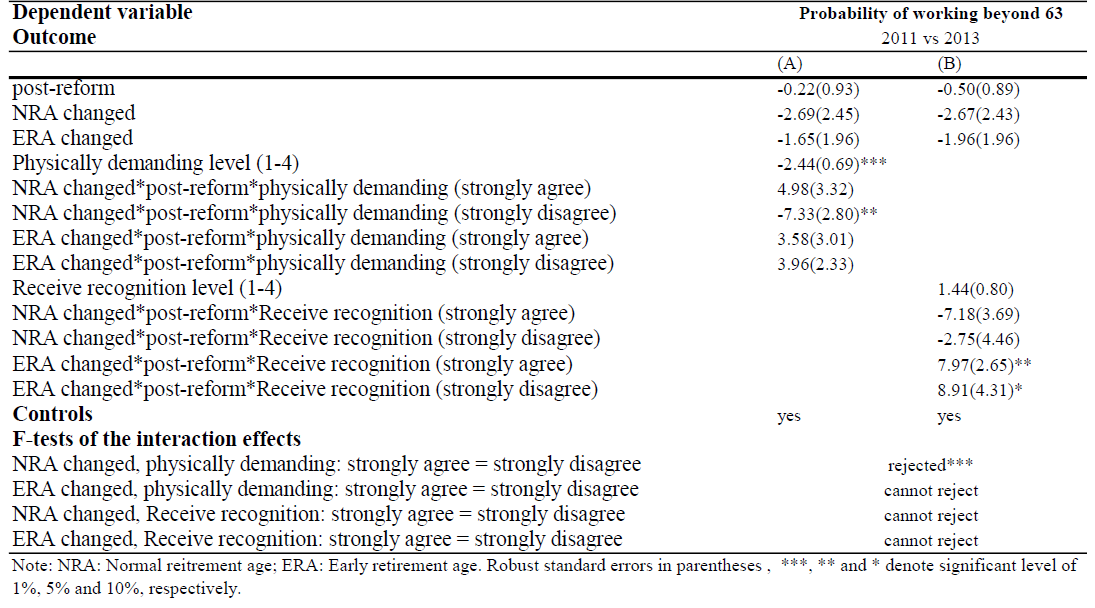
\includegraphics[width=1\linewidth]{table5.png}
    \caption{Difference-in-differences estimates, job level heterogeneity effects}
    \label{5}
\end{table}

There has been a general concern that whether the increases in pension ages are appropriate for workers who do physically demanding jobs and are usually forced to retire early because of the debility of body condition when approaching to an old age (Baily and Kirkegaard 2009). In this section we examine effect of pension reforms on workers’ retirement expectation, controlling for job characteristics or satisfaction—physically demanding and receive recognition—and their interaction with the reform dummy and the NRA/ERA treatment. Respondents in SHARE were presented by some statements that describe their present job and were asked to report (by strongly agree, agree, disagree or strongly disagree) how they feel about them. Table 5 reports the estimate results. 

As expected, higher level of physically demanding job reduces workers’ subjective probability to work beyond age 63 (by 2.44 percent per level). Although the effect of NRA reforms is not significant for those who reported ‘strongly agree’ to a physically demanding job state, it is for the workers who reported ‘strongly disagree’: A 7.3 percent decrease in the subjective probability is detected as their respond to the increases in NRAs. The divergence of responds is found to be significant at 1 percent level. However, increases in ERAs have no such effect on the retirement expectation after controlling the job heterogeneity. The results suggest that workers who perform a low physical intensity job can respond to the increase in NRA by shorten their expected work life, therefore substitution effects will prevail for them.

Column B of Table 5 show the heterogeneous treatment effects for receiving the recognition from the work. As can be seen, the influence of increases in NRAs on the subjective likelihood to work beyond age 63 is, statistically, insignificant and indifferent between group of ‘strongly agree’ and ‘strongly disagree’. For increases in EARs, both groups have responded by a substantial increase in their subjective working probability, amounting to 7.97 and 8.91 percent respectively. Again, the between-group difference is detected insignificant after conducting an F-test. 



\subsection{Quantile results}

We now turn to examine whether any effect of the pension reforms varies across the distribution of the subjective probability of working beyond age 63. In Figure 4, the x-axis values are the quantiles and the y-axis values denote the magnitude of specific coefficients. The black dashed line represents the value of OLS estimator along with 95 percent confidence interval indicated by the red dot line, and the solid line represents the quantile estimator with 95 percent confidence interval indicated by the grey area. 

\begin{figure}[h] 
    \centering
    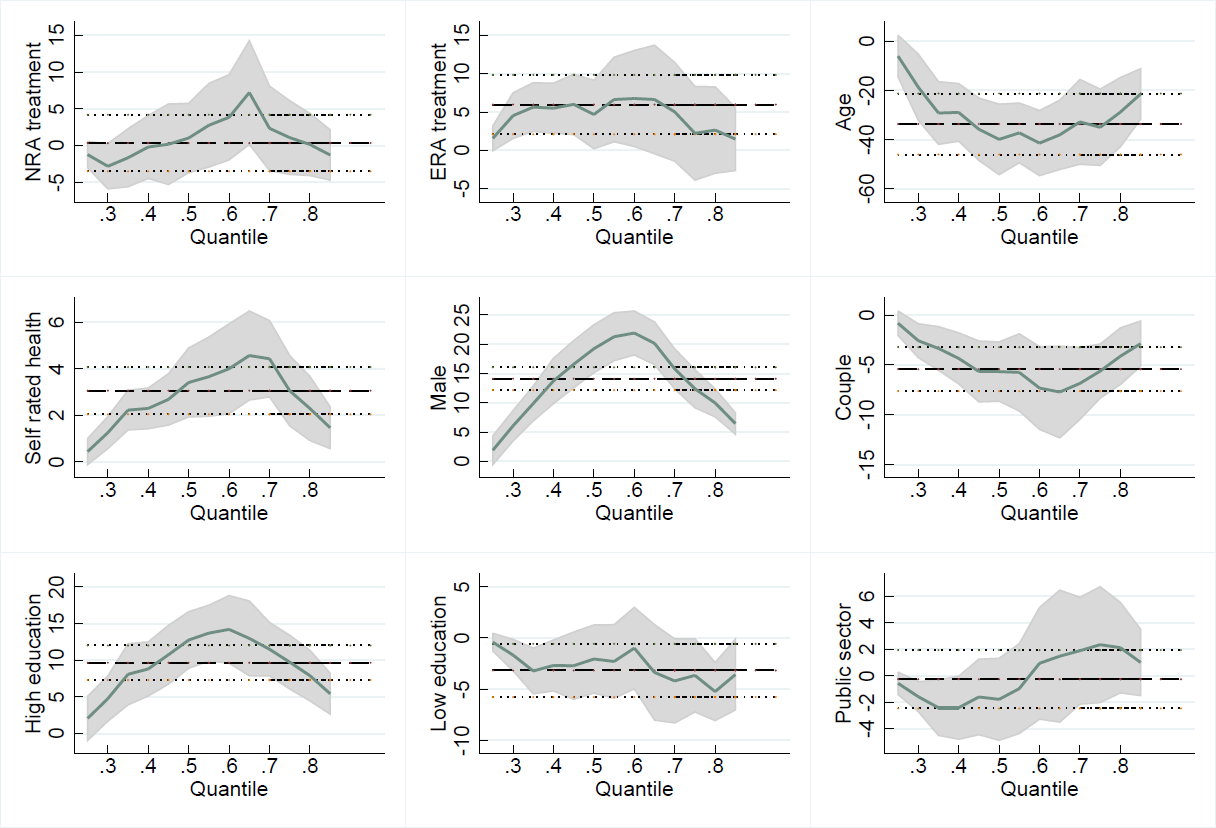
\includegraphics[width=1\linewidth]{figure3.png}
    \caption{Probability of working after 63 quantile regression results}
    \label{3}
\end{figure}

The result in the first panel show that changes in the subjective probability of working beyond age 63 caused by the increases in NRAs shape like an inverse ‘U’, as individuals of quantiles close to the middle part expected greater changes. However, except for the 0.65 percent quantile, the point estimate for other quantiles are not statistically different from the OLS estimator, and none of them are significantly different from zero. For the ERA treatment (shown in the second panel), the size of the effects is similar across quantiles form 0.3 to 0.7 percent and are consist to the mean estimates, whereas the two tails drop under the lower bond of mean interval and are no significantly different from zero. The patterns seen in both cases suggest that individuals who do not have a certain retirement plan (belongs to the middle quantiles) are more likely to respond to changes in retirement ages. Beside the policy factors, quantile effect across different individual characteristics is mostly significant under a similar pattern, except the “low education” dummy and “public sector” dummy. Note that the OLS estimates of “low education” and “public sector” variables are not significantly different from zero.



Previous results have shown strong average effect from raising the ERAs, as well as heterogeneous effects across education level, age cohort and whether performing a physically demanding job from raising the NRAs on individuals’ retirement preference. Comparing to the existing literatures, our findings opposite to the universal push-up power of raising the state pension ages on working intention. In fact, individuals of certain characteristics are able to respond with a declined subjective probability of working beyond age 63 when NRA increases to a high level. A natural question is how individuals adjust to these increases in NRAs and ERAs. Evidences from previous literature (Manoli and Weber 2016) indicate that individuals would stay in their jobs longer, or switch to another job for a longer work age as ERA increases. However, little is known on how individuals adjust to increase in NRA, especially for those who expected a declined working potential. One possible explanation would be that they would exit the job before the post-reform NRA and bridge the gap with alternative security benefits.  

\subsection{Trend of expected pension claims}

To shed light on the adjustment mechanisms, we start by plotting the survival curves of expected pension claims for both sexes after NRA or ERA changes in Figure 4. The solid lines in the graphics represent the survival rate until the expected pension claim for the control groups and the dash lines represent that of the treated groups. As one can see from the graphs, the pattern of expected pension claim is similar across genders: the labour supply at first declines smoothly and then dives at age 60 and 65. By age 67, nearly all the workers would exit the labour market. The effect of raising the NRAs, examined in the upper panels, is relatively small, as both the control and treated individuals expect similar age of pension claim. Especially for women, the impact is ambiguous: the expected survival at first increased, and then declined by about 5 percent across the 61-64 interval, followed by another small increase as approach to age 67 and become unrecognizable afterward. The results address that individuals may have non-public normal pension to maintain a relative fixed expected pension claim age as NRA increases.   

\begin{figure}[h] 
    \centering
    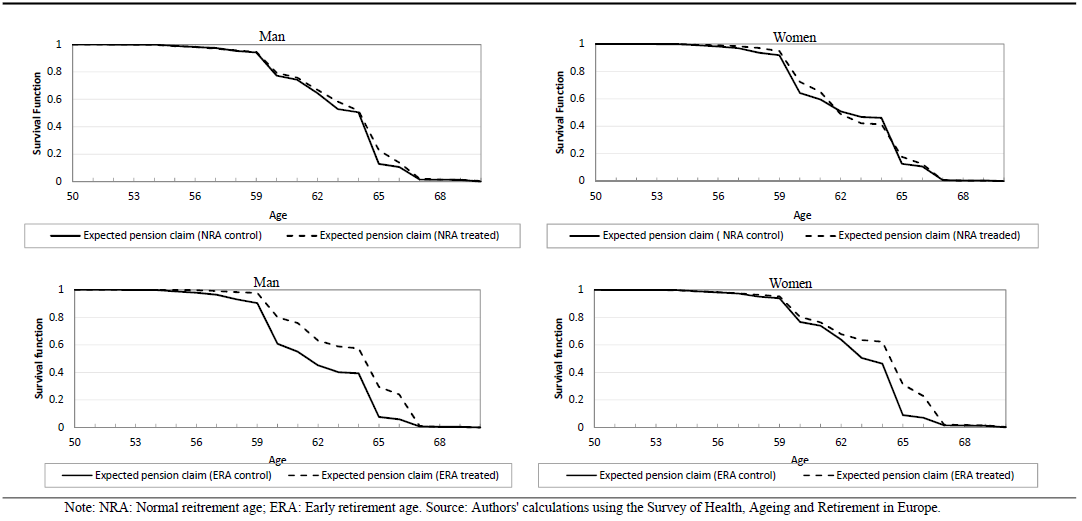
\includegraphics[width=1\linewidth]{figure4.png}
    \caption{Expected pension claim under NRA/ERA changes}
    \label{4}
\end{figure}

With that in mind, we now turn to the effect of increases in ERAs. Among man, shown in the left-bottom panel, the survival rate of pension claims increased significantly across 55-66 age interval as response to the increases in ERA and is at most 22 percent more (at age 65) than the rate of control group. A new dive point in pension claims is formed at age 67, whereas the drop at age 61 becomes smaller. Similar to men, we see pronounced shifts in the survival curve of women in the last panel. The difference between control and treated group starts to increase at age 62, reaching to a summit of 16 percent by age 65, and becomes negligible at age 67 and latter. Comparing across genders, the share of men who claim pension after age 59 increases with a greater magnitude after the raising of ERAs and becomes very close to that of the corresponding women. Notably, there is a substantial difference in expected pension claims between the two control groups (i.e. the NRA control group and ERA control group). While 36 per cent of men in the NRA control group expect to claim their pension prior to age 63, the corresponding number is more than 54 per cent for the ERA control group. 



\subsection{Entitlement of other pension plans}

Another way to investigate individuals’ ability to obtain alternative pension benefits. Table 9 reveals the impact of increasing the state pension ages on entitlement of’ non-public benefit plans, with heterogeneity check. The top row shows that as respond to the increased NRAs individuals are more likely to entitle social benefit plans other than public normal pension plan. In contrast, the estimated result of the impact of the increases in ERAs is small and insignificant. The table also shows that, interestingly, the gain of entitlement due to the increasing NRA is mostly significant among individuals aged between 54 and 61, or of lower education level. This could due to their low rate of entitlement in alternative pension at the base line year. Comparatively, the pre-retirement and high-educated individuals—who report declined subjective probability of working beyond age 63 after NRA increased—are of greater chance to entitle other pension plans before the reforms. These results suggest two insights. First, entitlement of pension other that public normal pension appears to have been a main technique for the old workers to respond to increases in NRAs. Second, older workers seem willing to prolong their work-life after affected by the increases in ERAs, as no change in alternative benefit plans is detected. 

\begin{table}
    \centering
    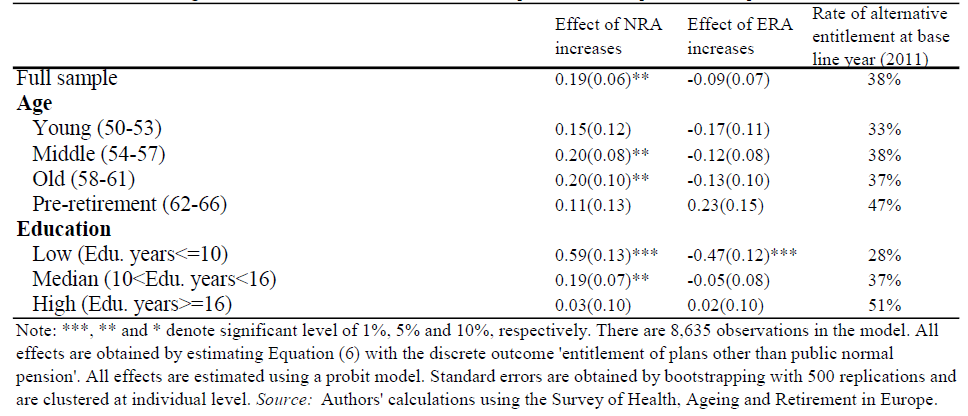
\includegraphics[width=0.9\linewidth]{table6.png}
    \caption{Effect of raising NRA or ERA on additional entitlement of plans other than public pension plans}
    \label{6}
\end{table}

\begin{comment}

\subsection{Unemployment after the reforms} 

Unemployment and Disability Insurance in many European countries can be used as financial support to cover the gap between the time of retirement and the time of actual claim of pension benefit. Li in 2017 developed a life-cycle model, where he incorporates both Disability Insurance and normal old-age pension to study the effect of increasing in the NRA (Li 2017). 

\begin{table}
    \centering
    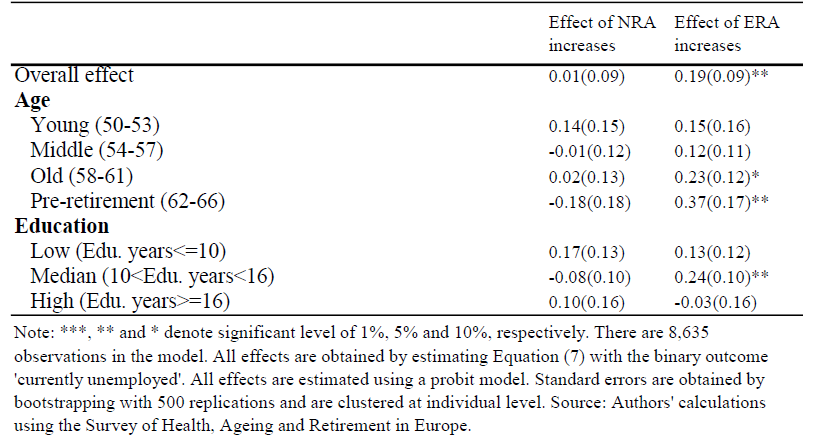
\includegraphics[width=0.9\linewidth]{table7.png}
    \caption{Effect of raising NRA or ERA on Unemployment}
    \label{7}
\end{table}

\end{comment}

\section{Conclusion}

This paper investigates the relationship between retirement expectation for individuals aged over 50 and the pension reforms issued during 2011 and 2013 across 10 European countries. In contrast to previous researches, we isolated the changes in NRAs and ERAs therefore are able to study their effects separately. To be specific, we first introduce a static labour supply model to theoretically describe how individual reacts under policy changes. We then quantify the effect of increases using repeated data collected in SHARE. The increases of NRAs and ERAs in the period of intense pension reforms are regarded as two separate treatments, and the effects of both are short-term due to the implement of reforms are shortly followed by our studying period. We identify the treated individuals using a self-generated approach which secures the exogeneity of the reforms, therefore the effects we report are likely to be causal.

Our quasi-experimental evidences show that the reforms in ERAs have significantly impact on individuals’ desire of prolonging their work life in short term, while the reforms in NRAs do not have such average effect. Considering the reforms in tightening the early retirement pathway are naturally stricter and usually include shape increases in pension ages, the results indicate that in short term individuals can respond to a substantial change in retirement legislation, however, have less reaction when reforms are gradual. After counting for heterogeneity, we find that the high-educated individuals revise to a greater intention of retirement early after the increase in NRA. The same pattern follows for the pre-retirement individuals, as they show a declined expected pension age under normal retirement reforms. These results suggest that a group of individuals are sticky with their initial retirement age. In order to counteract the cost of a higher pension age, workers would like to opt in alternative pension plans and become financially affordable to retire before the post-reform NRAs. This explanation is further supported by examining the changes in individuals’ entitlement of non-public pension plans, where a substantial increase in the likelihood of the entitlement is detected as respond to increase of NRA. Additionally, we examined the distributional treatment effects by estimating a quantile DiD model. We find that individuals who were not no certain about their retirement planning are more likely to respond to the increase in ERAs. Besides, we also studied the joint retirement decision of spouses. The results indicate that in short run changes in spouse’s legislated retirement age have little effect on both waves’ and husbands’ retirement expectation, as presented in appendix.

From policy point of view, our research suggests that the increases in ERA are effective in prolonging individuals’ expected working life in short period. Additionally, increases in ERA are powerful to the individuals with greater uncertainty. This would be crucial for countries that allocate different pension benefits between single and family retirement, since unpaired individuals usually face less uncertainty when planning retirement time. On the other hand, policy-maker should keep in mind that aggressive increases in NRA have starting to push individuals into alternative social benefit plans. Subsidies should be applied, to some extent, in order to make people feel “fair” about the changes in public normal pension age. 






\end{document}
